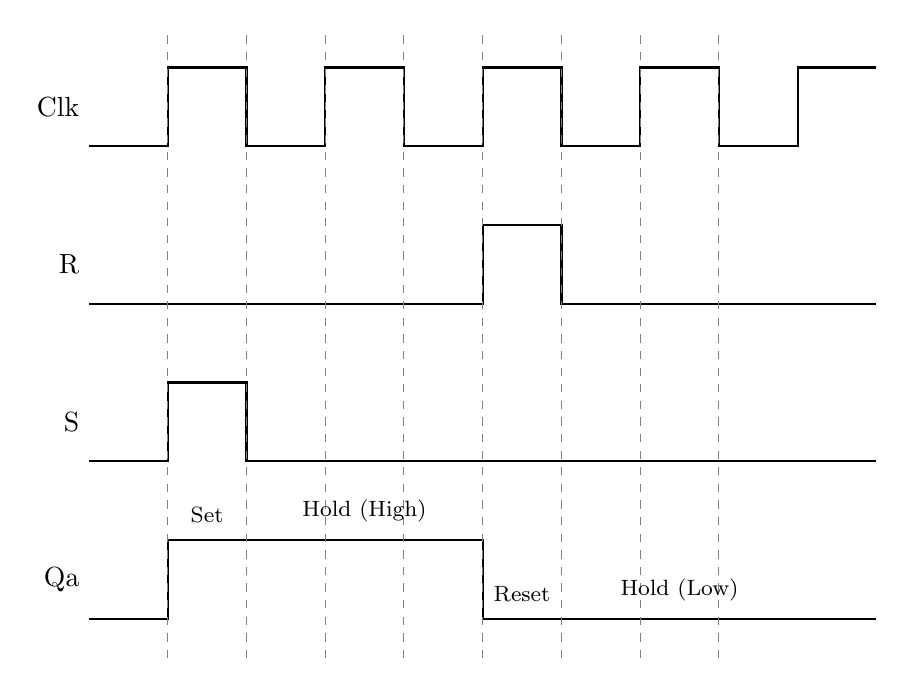
\begin{tikzpicture}[
    signal/.style={draw, thick},
    axis/.style={draw, ->},
    dashed_line/.style={draw, dashed, gray}
]
    % Define coordinates
    % Define coordinates
    \def\clkY{6}
    \def\rY{4}
    \def\sY{2}
    \def\qY{0}
    
    \def\maxX{10}
    
    % Labels
    \node[left] at (0, \clkY + 0.5) {Clk};
    \node[left] at (0, \rY + 0.5) {R};
    \node[left] at (0, \sY + 0.5) {S};
    \node[left] at (0, \qY + 0.5) {Qa};

    % Clock Signal (Toggling every 1 unit)
    \draw[signal] (0,\clkY) -- (1,\clkY) -- (1,\clkY+1) -- (2,\clkY+1) -- (2,\clkY) -- (3,\clkY) -- (3,\clkY+1) -- (4,\clkY+1) -- (4,\clkY) -- (5,\clkY) -- (5,\clkY+1) -- (6,\clkY+1) -- (6,\clkY) -- (7,\clkY) -- (7,\clkY+1) -- (8,\clkY+1) -- (8,\clkY) -- (9,\clkY) -- (9,\clkY+1) -- (10,\clkY+1);

    % R Signal (Reset)
    % Pulse High at t=5-6 (Reset)
    \draw[signal] (0,\rY) -- (5,\rY) -- (5,\rY+1) -- (6,\rY+1) -- (6,\rY) -- (10,\rY);

    % S Signal (Set)
    % Pulse High at t=1-2 (Set)
    \draw[signal] (0,\sY) -- (1,\sY) -- (1,\sY+1) -- (2,\sY+1) -- (2,\sY) -- (10,\sY);

    % Q Signal (Output)
    % 0-1: Hold 0
    % 1-2: Set -> 1
    % 2-3: Hold 1 (Clk Low)
    % 3-4: Hold 1 (Clk High, Inputs 0) -> "Hold High"
    % 4-5: Hold 1 (Clk Low)
    % 5-6: Reset -> 0
    % 6-7: Hold 0 (Clk Low)
    % 7-8: Hold 0 (Clk High, Inputs 0) -> "Hold Low"
    
    \draw[signal] (0,\qY) -- (1,\qY) -- (1,\qY+1) -- (5,\qY+1) -- (5,\qY) -- (10,\qY);

    % Dashed vertical lines at clock edges or transitions
    \foreach \x in {1, 2, 3, 4, 5, 6, 7, 8} {
        \draw[dashed_line] (\x, -0.5) -- (\x, \clkY+1.5);
    }
    
    % Annotations
    \node[above, font=\footnotesize] at (1.5, \qY+1.1) {Set};
    \node[above, font=\footnotesize] at (3.5, \qY+1.1) {Hold (High)};
    \node[above, font=\footnotesize] at (5.5, \qY+0.1) {Reset};
    \node[above, font=\footnotesize] at (7.5, \qY+0.1) {Hold (Low)};

\end{tikzpicture}
